% --------------------------------------------------------------------

\section{Abstract}
\label{sec:abs}

This report shows how MLP could be used in spam filtering context. We introduce ANN, PCA MLP, backpropagation, Gauss-Newton algorithm and its modification Levenberg-Maquardt optimization algorithm to a reader. We test MLP with data set of 10 000 email messages given on the course on Machine Learning. We show how PCA can be used to reduce the dimensions of a data set. We analyze our results and see how neural network is does not find the global optimum results for its model. MLP has a problem of reliability, which is discussed.

% --------------------------------------------------------------------

\section{Introduction}
\label{sec:intro}

In this paper we study how to filter spam using artificial neural network computing and how well does a neural network called multilayer perceptron perform in the task.

By spam we mean advertisement, virus-infected and fraud e-mail messages that we don’t want. If we can filter the spam from the meaningful e-mail we can reduce the need for repetitive human work. Good spam filtering enables better human productivity. Spam filters are not perfect. Sometimes spam gets in our inboxes despite of spam filters (false negative). On the other hand our meaningful mail may be lost because of false alarms of the spam filter (false positive) \cite{wiki:email} . 

Artificial neural networks are a bionic and connectionist approach to computing. In this paper we’ll be filtering spam with a multilayer perceptron (MLP) which is widely used for pattern recognition. Spam filtering is such a problem. We’ll look into MLP and its model parameters in detail with a mathematical approach \cite{wiki:mlp} . 

As a test set we have a table of boolean values (ones and zeros) of mail attributes. 448 columns represent the spam relevant attributes of the mail such as \verb!WEIRD_QUOTING! (weird repeated double-quotation marks), \verb!CHARSET_FARAWAY! (character set indicates a foreign language) or \verb!EMAIL_ROT13! (body contains a ROT13-encoded email address). The 10 000 rows represent 10 000 mails with different attributes. We have the information whether a mail is spam or not which we use to train our neural network.

We’ll see that MLP works as a spam filter but does not in itself reach a commercial level.


% --------------------------------------------------------------------

\section{Methods}

\subsection{Principal Component Analysis (PCA)}
\label{sec:pca}

Principal component analysis (PCA) \cite{wiki:pca} is a method used for analysing input data. This method can be also used to decrease the dimensionality of the data, which reduces the amount of computation needed in later processes. This method adds more error to learning algorithms as the data is represented in smaller space, which is a major drawback.

Process of decreasing the dimensions for a given data consists of 5 stages. Data is comprised of N samples of d-dimension vectors. We aim to have $p$ dimensions in the end of the process.

1. Data vectors are centered around the origin. This step is needed for calculating covariance matrix correctly.

2. Covariance between the attributes is calculated into a covariance matrix $C$ from the data.

3. Eigen values and corresponding eigen vectors of the matrix is calculated. It has been proven \cite{luentokalvo} that eigen vector created from the largest eigen value is a vector showing the direction of largest variance inside the data set.

4. Create a matrix $W$ from the eigen values corresponding to the $p$ largest eigen values.

5. Project each data point used in the system to vector space $p$ by calculating \[ z^i = W^Ty^i \] Where $z^i$ is the new calulated point.

As proportion of variance increases when number of dimensions increase, there is an trade off of choosing a small $p$ and a high additional error. Proportion of variance can be calculated using the formula

\[ PoV(k) = \sum_{i=1}^p\lambda_i/\sum_{i=1}^d\lambda_i \]

Appropriate $p$ is selected depending on the shape of PoV function and other requirements on accuracy.

\subsection{Artificial Neural Networks (ANN)}
\label{sec:ann}

An artificial neural network (ANN) consists of an interconnected group of artificial neurons, and it processes information using a connectionist approach to computation \cite{wiki:nn}.



\begin{figure}[h]
  \centering
  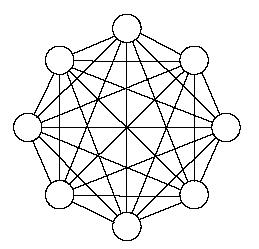
\includegraphics{hopfig}

  \caption{Hopfield Neural Network}
  \label{fig:hopfield}
\end{figure}



In the picture we see a simple neural network. The circles are the neurons and the lines are the connections between the neurons. Neurons have one or more inputs and only one output which, however, can be connected to multiple neurons. A neuron computes the information from its inputs into an output \cite{wiki:nn} . 

\subsection{Feedforward Neural Networks (FFNN)}
\label{sec:ffnn}

A feedforward neural network (FFNN) is an artificial neural network where the connections between the neurons do not form a directed cycle \cite{wiki:ffnn}.

\begin{figure}[h]
  \centering
  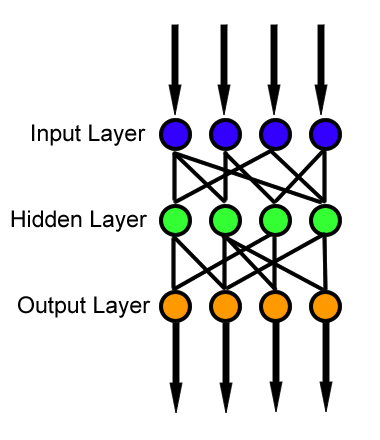
\includegraphics[width=6cm,keepaspectratio=true]{ffnn}
  \caption{Simple feedforward neural network}
\end{figure}
Simple feedforward neural network


As we can see in the picture the information flows to a single direction. Feedforward neural networks usually have layers of neurons:

\begin{enumerate}
\item Input layer
\item Hidden layers (if any)
\item Output layer
\end{enumerate}

Each input and output neuron corresponds to one input or output of the network  \cite{wiki:ffnn}

One hidden layer is usually the best choice and in most cases adding more hidden layers does not improve performance at all \cite{ham2001} .

\subsection{Multilayer Perceptron}
\label{sec:mlp}

A multilayer perceptron (MLP) is a feedforward neural network and the standard algorithm for any supervised-learning pattern recognition process \cite{wiki:mlp}

\begin{figure}[h]
  \centering
  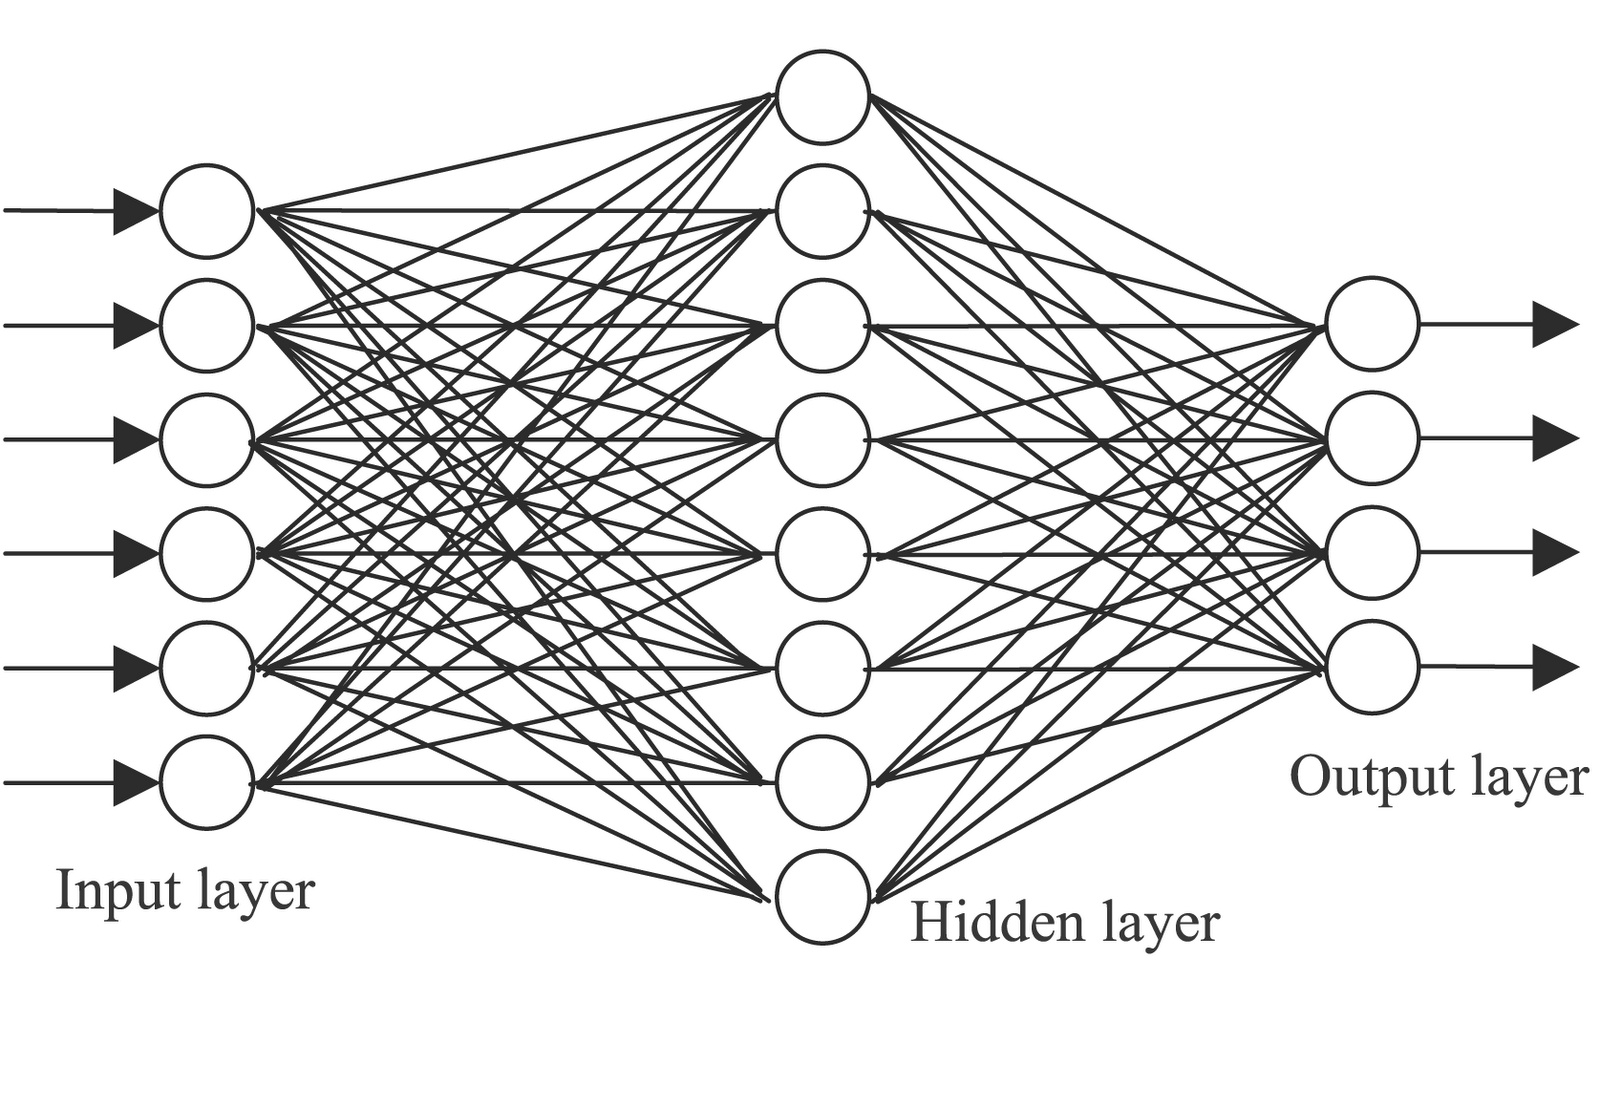
\includegraphics[width=8cm]{mlp}
  \caption{Multilayer perceptron}
\end{figure}

As we can see in the picture a multilayer perceptron is a feedforward neural network where each neuron of each layer takes an input from each neuron of the previous layer. Input layer neurons handle only one network input each.


\subsubsection{Backpropagation}
\label{sec:backprop}

Multilayer perceptron utilizes a supervised learning technique called backpropagation for training the network. Backpropagation consists of two phases that are repeated through the training set. Iterations of these phases are called epochs. As many epochs are run as it is needed to find a local minimum in the error function or until we’re out of training data.  \cite{wiki:mlp} \cite{wiki:backprop} , )

\paragraph{Phase 1: Propagation}

Let $m = 0, 1, …, M$ be the layer index. 0 stands for the input layer and $M$ for the output layer. Denote $a_i^m, i = 1, 2, …, k[m]$ the output signals of the $m$-th layer neurons. It is convenient to use zero indices for the bias signal; then always we have $a_0^m = 1$. A neuron’s output signal $a_i^m$ is calculated as following:

\[ h_i^m = \sum_{j=0}^{k[m-1]} w_{i,j}^m * a_j^{m-1} \]

Where $i = 1, 2, …, k[m]$ is the neuron’s index, $j = 0, 1, …, k[m-1]$ are the indeces of the previous layer’s neurons’ output signals (the inputs for the current neuron) and $w_{i,j}^m$ is the weight for the input. For the first epoch the weights can be chosen by random.

\[ a_i^m = f^m(h_i^m) \]

Where $f^m$ is the activation function. Activation function is usually sigmoid such as hyperbolic tangent.

Let $l = 1, 2, …, L$ be the index of the current epoch. Let’s consider the l-th sample of the training set. For inputs we have an array $a_i^0 = P_{l,i}$. Then let $T_{l,i}$ be the array for wanted outputs. Cost function for the $l$th sample is:

\[ F_l(W) = \frac{1}{2} \sum_{i=1}^{k[M]} e_li^2 = \frac{1}{2} \sum_{i=1}^{k[M]} (a_i^M - T_{l,i})^2 \} \]

Where $W$ consists of all the weights of the network.

Then we’ll calculate the so-called deltas iterating backwards starting from the network output i.e. the $M$th layer:

\[ \delta_i^M = (f^M)’(h_i^M)*(a_i^M - T_{l,i}) \]

For other layers we calculate:

\[ delta_i^{m-1} = (f^{m-1})’(h_i^{m-1}) \sum_{j=1}^{k[m]} w_{i,j}^m*\delta_i^m \]

\subsubsection{Phase 2: Weight update}

Let’s calculate the derivatives for $F_l(W)$:

\[ g_{i,j,l}^m = delta_i^m * a_j^{m-1} \]

The derivatives are the entries of the gradient:

\[ g_l(W) = \nabla_w F_l(W) \]

Having the values of $g_l(W)$ we can update $W$ with incremental learning:

\[ (w_{i,j}^m)^{new} = (w_{i,j}^m)^{old} - \alpha g_{i,j,l}^m \]

Where $\alpha$ is the learning rate parameter. $\alpha$ can be a small constant or we can use heuristic algorithms to optimize $\alpha$ for each epoch.

We want to minimize the sum of cost functions:

\[ f(W) = \sum_{l = 1}^L F_l (W) \]

Then

\[ g(W) = \nabla_w f(W) = \sum_{l = 1}^L g_l (W) \]

and

\[ g_{i,j}^m = \sum _{l = 1}^L g_{l,i,j}^m \]

 \cite{hongwei} \cite{wiki:mlp} \cite{wiki:backprop}


\subsubsection{Model Parameters}

While MLP is one of the simplest ANN model used in machine learning, it is a complex system with a number of parameters to choose from.

1. Number of hidden layers and size of them in neurons should be selected \cite{hiddenunits} .  Size of the MLP is proportional to its model complexity, and in general avoiding over and under fitting is preferred. Additional neurons increase the computation needed for the ANN. There are no methods to define these two parameters \cite{hiddenunits} . Finding appropriate number for hidden layers and their neurons is an iterative process. In our experiments \ref{exp:hidden} we did not notice any improvement in accuracy  with extra layers or neurons.

2. Activation function in a neuron define the output of the neuron from the weighted inputs. Selecting a activation function for each neuron, or layer,  changes general behavior of the ANN, what outputs the ANN gives and how learning function acts. There exists several different activation functions, some of which are shown in the figure x. Activation functions should work hand in hand with the chosen training function. For example backpropagation requires activation functions to be differentiable. We chose all activation functions to be hyperbolic tangent functions as we figured they should work well with every kind of data.

3. Teaching is a process where an weight vectors of an ANN are modified to make the network predict output more accurately. While backpropagation is bases on layer to layer propagation, in section \ref{mlp:backprop}  we showed that backpropagation can be formulated as an optimization problem, where combined error function for all the given weights W:

\[f(W) = \frac{1}{2} e^Te,\]

where $e$ is an vector consisting of every output from every teaching sample. This enables us to use several different optimization methods, such as  Gauss-Newton Algorithm (GNA), which updates the weight values by calculating second-order approximation of derivate of function $f(W)$, and then approximating Hessian matrix $H(x) \approx J^T(x)J(x)$:

\[ W_{i+1} = W_i +  [J^T(x)J(x)]^{-1}J^T(x) * e \]

We chose to use Levenberg-Marquardt teaching algorithm (LMA) as it is more robust than GNA. While GNA is very accurate method in most of the cases, but with large residuals $J^T(x)J(x)$ is not invertible. LMA modifies GNA by adding a term $\mu I$ to the approximation of hessian matrix:

\[ H(x) \approx J^T(x)J(x) + \mu I \]

$\mu I$ causes the approximation to become a positive definite matrix, a property required for calculating $H^{-1}(x)$. $\mu$ is  called dampening factor in literature, sometimes denoted by $\lambda$. $\mu$ is adjusted so that it is as small as possible. Matlab does the adjustment in powers of 10. With small values of $\mu$ Hessian matrix in LMA is approximately same as  the one used in GNA making LMA to act like GNA in close vicinity of the local minimum.


\subsection{Advantages and disadvantages of Multilayer Perceptron}

Multilayer perceptrons differs from other supervised classifiers by being able to learn and classify online \cite{wiki:onlinealgorithm} ,  by one data point at a time. This makes it practical in many engineering tasks, such as when data cannot be stored.

It is currenty impossible to analyze neural networks on what they have learned showing how they work as a black box. This introduces risks to a system.


\section{Experiments}

We created our machine learning model using MATLAB    , software for numerical computation, and its Neural Network Toolbox  \cite{matlab:nn} .

Input data, which were test results of 10000 different email messages, were represented in  binary vectors, where each value represent the output of a single email analyzer test. As vector space was quite large, $\{0,1\}^{448}$, we needed to reduce the dimensionality by using PCA. to speed up the process of learning.

In MATLAB, PCA algorithm has been implemented as one function, \verb!princomp!, which takes input data as a parameter, and returns a matrices of eigen vectors and eigen values. We calculated proportion of variance for different values of $p$ and chose $p$ where its PoV was at least 0.95.

Neural Network Toolbox provides data structures for MLP, including different activation functions (denoted as transfer functions in the toolbox) and teaching functions. This left us to work on understanding on how to use the toolbox and to make correct decisions on learning model selection. Documentations of the toolbox were not comprehensive and it seemed to be doing some assumptions and setting default parameters which we were not aware of.

Toolbox handles teaching and test data differently than in other machine learning methods as teaching in MLP happen one data point at a time. Toolbox then allowed us to divide the points into training, validation and test samples. However, toolbox did not give information on what it does with the validation data. We do not know what kind of model selection happens in this process. We divided our 10000 samples to echo real life scenario, where test emails are abundant relative to the emails used in teaching, granted creating teaching data for spam filter is not costly. See figure y for our division sizes.

We ran repetitive tests on how well networks with different number of hidden neurons perform. L-M training algorithm consumes a lot of memory so we were limited to maximum of 10 hidden neurons. Tests were run with numbers from 1 to 10 hidden neurons. We noticed that 14\% of the times a network was trained the training failed and the network marked every mail as spam. We ignored the networks with worse than 90\% accuracy.

The Levenberg-Marquardt is very sensitive to the initial network weights and it does not consider outliers in the data which may lead to overfitting noise  \cite{crsouza} . This may be the reason training the network fails in 14\% of the times.

The teaching time of the network increases quickly when more hidden neurons are added. With current computers it usually takes less than ten seconds to teach a network with a few hidden neurons and some minutes with tens of hidden neurons. However, when the network is taught, testing single mails does not load system much at all.

We chose our activation function to be a hyperbolic tangent, which worked well with the Levenberg-Marquardt teaching algorithm. Our focus was not on finding the optimal activation function as most of the studying material did not contain any mention on how to proceed. We considered on using GNA as error values used in our training should not be large ( training values alternate between zero and one).

MLP outputs values in rational numbers, and we transform them to binary by using treshold 0.5.

\section{Results}
\label{sec:results}

\begin{figure}[h]
  \centering
  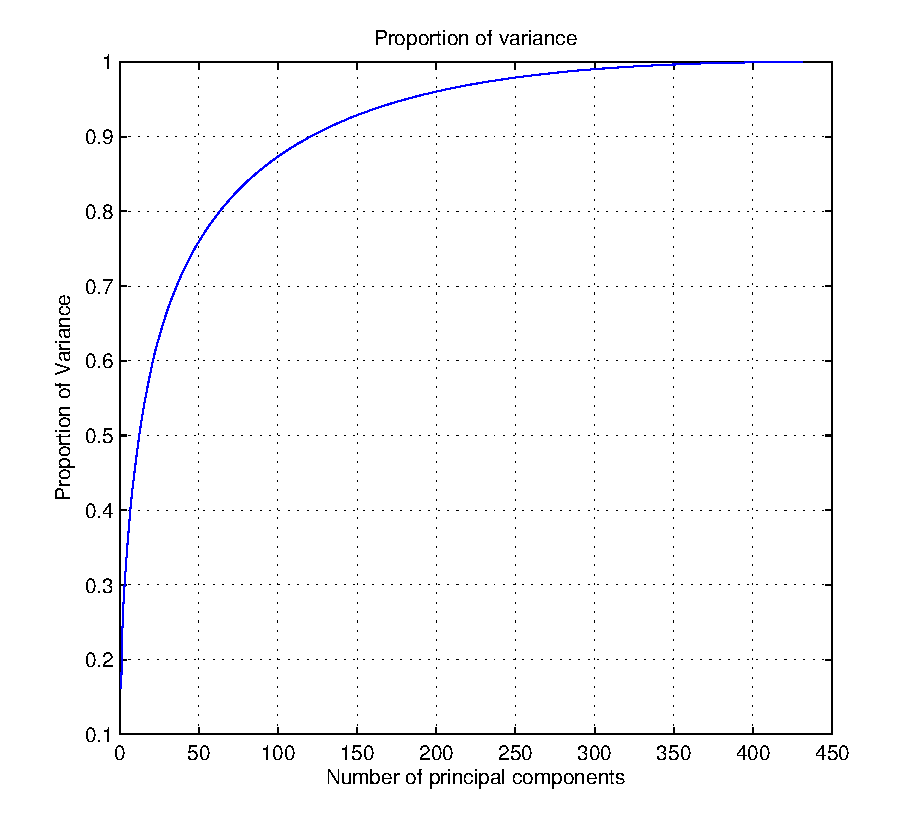
\includegraphics{pov}
  \caption{Proportion of Variance}
\end{figure}

We can see the elbow point of the curve around 0.8. We kept 64 of the 448 dimensions to keep 80\% of the information in our newly modified data.

\begin{figure}[h]
  \centering
  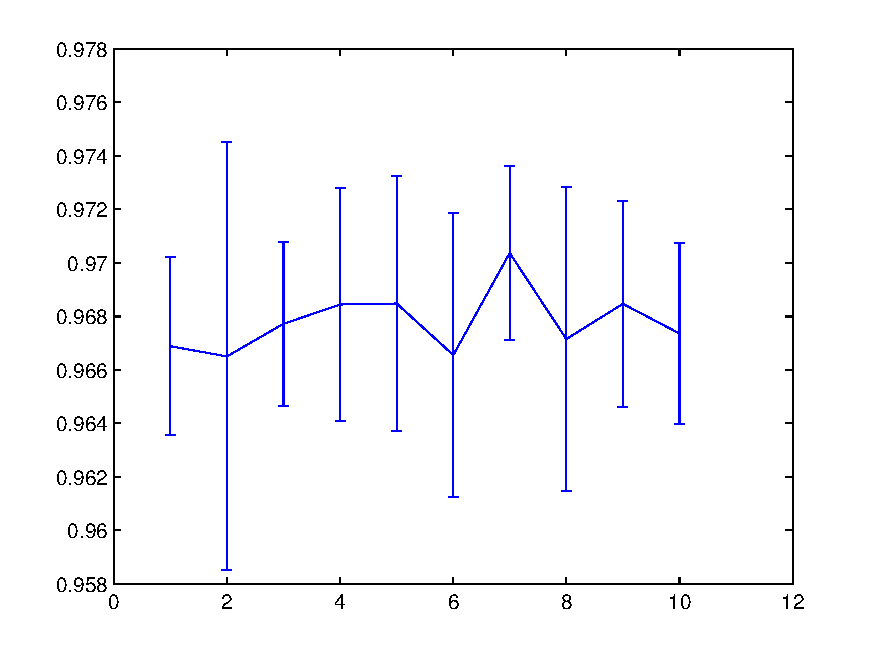
\includegraphics{hidden_neurons_are_useless}
  \caption{Proportion of Variance}
\end{figure}


Our tests with variable sized hidden layer showed how increasing the network size does not improve the classification. For the final tests our model had one hidden neuron in one hidden layer.

\begin{figure}[h]
  \centering
  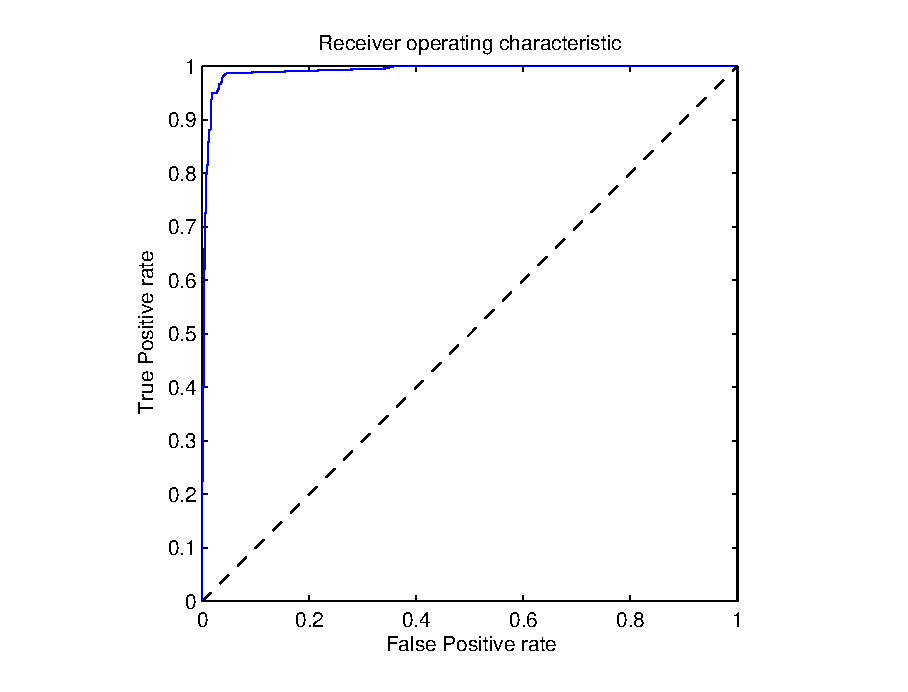
\includegraphics{roc}
  \caption{Proportion of Variance}
\end{figure}

\begin{figure}[h]
  \centering
  \begin{tabular}[h]{|c|c|}
    \hline
    True Negative = 3273 & False Negative = 250 \\
    \hline
    False Positive = 93 & True Positive = 6384\\
    \hline

  \end{tabular}

\end{figure}

\begin{center}
  \begin{tabular}[h]{ll}
    Accuracy & 0.9657 \\
    Error rate & 0.9623 \\
    Hit rate & 0.9623 \\
    False alarm rate & 0.0276
  \end{tabular}
\end{center}



\begin{figure}[h]
  \centering
  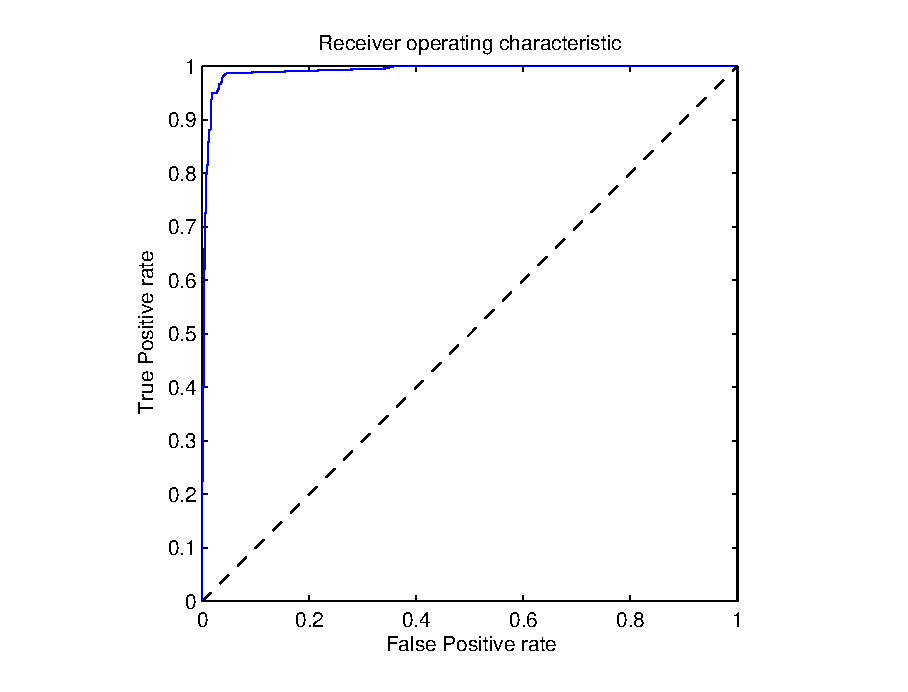
\includegraphics{roc}
  \caption{Proportion of Variance}
\end{figure}





From ROC curve we can see that the neural network is not guessing.

\clearpage
\section{Conclusions}
\label{sec:conclusions}

In general we can say that MLP can learn to filter spam, or it can be used as a part of the filtering system. Some of our training attempts failed for an unknown reason, which should be looked into in the future research. The only random selection in the teaching process happens when selecting the initial weights.

Results show that the hypersurface of overall error has many local minima.  Finding a global minimum is practically impossible in this setup. Bayesian Regularization could be one of the tools to reduces this noise \cite{crsouza} .

Our figure of proportion of variance with different number of principal values showed the characteristic elbow point seen in most of every real life data.

It was expected that these results could not be perfect when using one single model for classifying. Accuracy of 96\% is a decent value when comparing to other students who operated on the same data  \cite{datachallenge} . Still, MLPs of this form might not be the best ones to use in spam filtering, when taking account other disadvantages of the MLP. Classifier achieving same or greater results can be done more easily using Bayesian models. In conclusion, MLP classifier was a little too big task for us to analyze in this report.

Advantages of MLP are better used on tasks where training samples are more scarce and where teaching has to be done online or the teaching is otherwise costly.

Adding hidden neurons and layers is still a mystery, which should be researched more carefully in the future.







